%% grouprank.tex - Computing group rank with limited nondeterminsm
%%
%% Copyright 2014, 2015 Jeffrey Finkelstein.
%%
%% This LaTeX markup document is made available under the terms of the Creative
%% Commons Attribution-ShareAlike 4.0 International License,
%% https://creativecommons.org/licenses/by-sa/4.0/.
\documentclass{article}

\usepackage{amsmath}
\usepackage{amssymb}
%% This must come before hyperref.
\usepackage{amsthm}
%% This is strongly recommended by biblatex.
\usepackage[english]{babel}
\usepackage[backend=biber]{biblatex}
\usepackage[T1]{fontenc}
%% This must come before csquotes.
\usepackage[utf8]{inputenc}
\usepackage{lmodern}
%% This is strongly recommended by biblatex.
\usepackage{csquotes}
%% This must come before hyperref.
\usepackage{thmtools}
%% This must come before complexity.
\usepackage{hyperref}
\usepackage{complexity}
\usepackage[firstpage]{draftwatermark}
\usepackage{microtype}
\usepackage{textcomp}
\usepackage{tikz}

\usetikzlibrary{trees}

\LoadMicrotypeFile{cmr}
\SetProtrusion
    [load=lmr-T1]
    {encoding=T1, family=lmr}
    {
      \textquotedblright = {,1000},
      \textquotedblleft = {1000,},
      {'} = {,1000},
      {,} = {,1000},
      {:} = {,1000},
      {;} = {,1000},
      {.} = {,1000}
    }


%% Set the ``work-in-progress'' watermark for the first page.
\SetWatermarkLightness{0.9}
\SetWatermarkText{Work-in-progress}
\SetWatermarkFontSize{3.5cm}

%% Set the title and author of the PDF file.
\hypersetup{pdftitle={Computing group rank with limited nondeterminism}, pdfauthor={Jeffrey Finkelstein}}

%% Declare the bibliography file.
\addbibresource{grouprank.bib}

%% Declare theorem-like environments.
\declaretheorem[]{theorem}
\declaretheorem[numberlike=theorem,style=definition]{example}
\declaretheorem[numberlike=theorem]{corollary}

%% Custom commands are declared here.
\newcommand{\email}[1]{\textlangle\href{mailto:#1}{\nolinkurl{#1}}\textrangle}
\newcommand{\todo}[1]{\textbf{TODO #1}}

%% Redefine the footnote environment so it has no reference and no number.
\long\def\symbolfootnote#1{\begingroup%
\def\thefootnote{\fnsymbol{footnote}}\footnotetext{#1}\endgroup}

%% Define the author, title, and date for the document.
\author{Jeffrey~Finkelstein\\ Computer Science Department, Boston University}
\title{Computing group rank \\ with limited nondeterminism}
%\date{\today}

\begin{document}

\maketitle

\symbolfootnote{%
  Copyright 2014, 2015 Jeffrey~Finkelstein \email{jeffreyf@bu.edu}.

  This document is licensed under the Creative Commons Attribution-ShareAlike 4.0 International License, which is available at \mbox{\url{https://creativecommons.org/licenses/by-sa/4.0/}}.
  The \LaTeX{} markup that generated this document can be downloaded from its website at \mbox{\url{https://github.com/jfinkels/grouprank}}.
  The markup is distributed under the same license.
}

\section{Introduction}

An efficient algorithm computing the rank of a group (that is, the size of a minimum generating subset) benefits mathematicians, who use numerical algebra systems for research, cryptographers, who rely on algebraic systems for proofs of security, and theoretical computer scientists, who seek to understand which problems can be solved in a particular model of computation.
Before now, the best algorithm for computing the rank of a group required a polylogarithmic amount of space, which induces a superpolynomial (hence, inefficient) algorithm.
We reduced the best upper bound on the complexity of the group rank problem and provide a theoretically efficient algorithm for it.
This paper proves that with very short certificates of correctness, the group rank problem can be verified by highly restricted models of computation.

We prove that the problem of deciding whether the rank of a finite group, given as a multiplication table, is smaller than a specified number is decidable not only by a circuit of depth $O(\log \log n)$ augmented with $O(\log^2 n)$ nondeterministic bits, but also by a Turing machine using $O(\log n)$ space and $O(\log^2 n)$ bits of nondeterminism.
These models of computation are extremely limited in computational power, and hence can be simulated by a deterministic Turing machine in polynomial time.
Using limited nondeterminism and restrictive models of computation as verifiers may also be useful in examining other algebraic problems.

The limited nondeterminism lens suggests some opportunities for further research in computational algebra.
Is computing the rank of a quasigroup, a problem more general than computing the rank of a group, in $\bL$ as well?
Is there a reduction between the problem of computing the rank of a quasigroup and the problem of deciding whether two quasigroups are isomorphism?
Finally, is the problem of computing a minimum generating sequence for a quasigroup strictly more difficult than the problem of computing the rank of a quasigroup?

\section{Preliminaries}

\L{} is the class of languages decidable by a deterministic Turing machine that uses $O(\log n)$ space on inputs of length $n$.
$\L^2$ is the class of languages decidable by a deterministic Turing machine that uses $O(\log^2 n)$ space.
\NL{} is the class of languages decidable by a nondeterministic Turing machine that uses $O(\log n)$ space.
$\bL$ is the subclass of \NL{} in which the nondeterministic Turing machine uses at most $O(\log^2 n)$ nondeterministic bits.
\FOLL{} is the class of languages decidable by a \L-uniform family of circuits with polynomial size, unbounded fan-in, and $O(\log \log n)$ depth.
$\bFOLL$ is the class of languages decidable by \FOLL{} circuits that have been augmented with $O(\log^2 n)$ nondeterministic bits (gates with no inputs and one output).
In general, the class $\beta_2 \mathcal{C}$ is the class of languages decidable by $\mathcal{C}$ machines augmented with $O(\log^2 n)$ bits of nondeterminism.
%%$\NC^2$ is the class of languages decidable by a \L-uniform family of circuits with polynomial size, fan-in 2, and $O(\log^2 n)$ depth.

A \emph{quasigroup} is a set $G$ with a binary operation $\cdot$ such that for each $a$ and $b$ in $G$ there exist unique elements $x$ and $y$ in $G$ such that $a \cdot x = b$ and $y \cdot a = b$.
(In other words, each quasigroup element appears exactly once in each row and each column of the multiplication table of $G$.)
If the quasigroup is nonempty and associative, then it is a \emph{group}.

\begin{example}\label{ex:quasigroup}
  The smallest quasigroup that is not also a group has three elements, $\{a, b, c\}$.
  Its multiplication table is
  \begin{equation*}
    \begin{array}{c | c c c}
      \cdot & a & b & c \\
      \hline
      a & a & b & c \\
      b & c & a & b \\
      c & b & c & a \\
    \end{array}
  \end{equation*}
  This quasigroup is not associative because $b \cdot (a \cdot b) = b \cdot b = a$ but $(b \cdot a) \cdot b = c \cdot b = c$.
  Also, it has a left identity, $a$, but no right identity.
\end{example}

A \emph{parenthesization} $P$ of a sequence of quasigroup elements $(g_0, \dotsc, g_k)$ is a binary tree that has the quasigroup elements as its leaves (in the order indicated by the sequence).
The \emph{parenthesized product} of a sequence of quasigroup elements $(g_0, \dotsc, g_k)$ with parenthesization $P$, denoted $P(g_0, \dotsc, g_k)$, is the quasigroup element that results from performing the quasigroup product in the order indicated by the parenthesization.

\begin{example}
  Consider $(a, c, a, b)$, a sequence of four elements from the quasigroup defined in \autoref{ex:quasigroup}.
  One parenthesization of this sequence is
  \begin{equation*}
    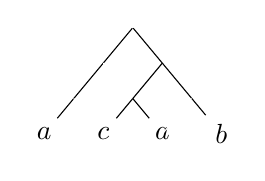
\begin{tikzpicture}[xscale=0.5, yscale=0.3]
      \node[minimum size=0pt, inner sep=0pt] {}
      child {
        child {
          child {node {$a$}}
          child[color=white] {}
        }
        child[color=white] {}
      }
      child {
        child {
          child {node {$c$}}
          child {node {$a$}}
        }
        child {
          child[color=white] {}
          child {node {$b$}}
        }
      };
    \end{tikzpicture}
  \end{equation*}
  which corresponds to the parenthesized product $a \cdot ((c \cdot a) \cdot b)$.
  According to the multiplication table, this product equals $a$.
\end{example}

A \emph{generating sequence of size $k + 1$} of a quasigroup $G$ is a finite sequence $(g_0, \dotsc, g_k)$ with a corresponding parenthesization $P$ such that
\begin{equation*}
  G = \left\{P(g_0, g_1^{\epsilon_1}, \dotsc, g_k^{\epsilon_k}) \, \middle| \, \epsilon_i \in \{0, 1\} \text{ for each } i \right\}.
\end{equation*}
The \emph{rank} of a quasigroup is the length of a minimum generating sequence.
If the quasigroup is a group, the operation is associative, so the parenthesization is superfluous, and the rank is simply the size of a minimum generating set.
If $S$ is a subset of group elements, the \emph{subgroup generated by $S$}, denoted $\langle S \rangle$, is the set of all group elements that can be expressed as a product of any number of elements of $S$.

\section{Efficient computation of quasigroup rank}

The \textsc{Quasigroup Rank} problem is defined as follows.
Given the multiplication table of a quasigroup and an integer $k$ in binary, decide whether the rank of the quasigroup is $k$ or less.
The \textsc{Group Rank} problem is defined similarly.

The \textsc{Quasigroup Isomorphism} problem is the problem of determining whether there is a bijection between two quasigroups (again, given as multiplication tables) that preserves the quasigroup operation.
This problem is in $\bFOLL$ \autocite[Theorem~3.4]{ctw13}.
Implicit in that algorithm is a $\bFOLL$ algorithm for \textsc{Quasigroup Rank}.

\begin{theorem}[{Implicit in \autocite[Theorem~3.4]{ctw13}}]
  \textsc{Quasigroup Rank} is in $\bFOLL$.
\end{theorem}
\begin{proof}
  By \autocite[Theorem~3.3]{ctw13}, each finite quasigroup with $n$ elements has a generating sequence of size $O(\log n)$ with a parenthesization of depth $O(\log \log n)$.
  The $\bFOLL$ algorithm works as follows on input quasigroup $G$ with $n$ elements (given as a multiplication table) and integer $k$, guaranteed to be in $O(\log n)$.
  \begin{enumerate}
  \item Nondeterministically choose a sequence of quasigroup elements $(g_0, \dotsc, g_k)$ and a parenthesization $P$ of depth $O(\log k)$.
  \item For each quasigroup element $a$, in parallel:
    \begin{enumerate}
    \item For each binary sequence $(\epsilon_1, \dotsc, \epsilon_k) \in \{0, 1\}^k$, in parallel:
      \begin{enumerate}
      \item Check if $P\left(g_0, g_1^{\epsilon_1}, \dotsc, g_k^{\epsilon_k}\right) = a$.
      \end{enumerate}
    \item Output $1$ if and only if some $(\epsilon_1, \dotsc, \epsilon_k)$ produces $a$.
    \end{enumerate}
  \item Output $1$ if and only if all elements of the quasigroup were produced.
  \end{enumerate}
  Since each quasigroup element can be represented using $O(\log n)$ bits, and since $k$ is in $O(\log n)$, this algorithm uses $O(\log^2 n)$ bits of nondeterminism to guess the generating sequence and parenthesization.
  %% TODO define FOLL and beta2 FOLL
  In step 2, there are $n$ group elements so we create $n$ parallel subcircuits.
  In step 2(a), since $k$ is in $O(\log n)$ there are a polynomial number of binary sequences of length $k$, so we create a polynomial number of parallel subcircuits.
  The innermost subcircuit that decides whether $P(g_0, g_1^{\epsilon_1}, \dotsc, g_k^{\epsilon_k}) = a$ requires a $O(\log \log n)$ depth circuit to compute the parenthesized product, plus a constant depth circuit to perform the equality comparison.
  In step 2(b), we use a single \textsc{or} gate (with unbounded fan-in).
  In step 3, we use a single \textsc{and} gate (with unbounded fan-in).
  Overall, the total size of this circuit is polynomial in $n$ and the depth is $O(\log \log n)$.
  The correctness of the circuit follows from the fact stated at the beginning of the proof, so we conclude that \textsc{Quasigroup Rank} is in $\bFOLL$.
\end{proof}

This theorem gives an immediate improvement over the previous best upper bound for \textsc{Group Rank}, which was $\L^2$ \cite{lsz77} (see \cite[Proposition~3]{at06} for a brief description of the algorithm).
%$\L^2$ is the class of languages decidable by a deterministic Turing machine using $O(\log^2 n)$ space.

\begin{corollary}\label{cor:grouprank}
  \textsc{Group Rank} is in $\bFOLL \cap \bL$.
\end{corollary}

\autoref{fig:inclusions} shows the chain of inclusions that demonstrates how great an improvement this is.
This also immediately improves the result of \cite[Theorem~7]{at06}, which shows \textsc{Nilpotent Group Rank} is in \P, since
$$
(\bFOLL \cap \bL) \subseteq \NL \subseteq \P.
$$
However, the relationship between \FOLL{} and \L{} remains unknown (the best inclusion known is the uninteresting inclusion $\FOLL \subseteq \AC^1$), so the relationship between $\bFOLL$ and $\bL$ is unknown as well.

\begin{figure}
  \caption{\label{fig:inclusions}$\bFOLL \cap \bL$ is much smaller than both $\L^2$ and \P.}
  \begin{center}
    \begin{tikzpicture}
      \node at (2, 4) (h) {$\P$};
      \node at (0, 6) (g) {$\L^2$};
      \node at (0, 5) (f) {$\bNC^2$};
      \node at (0, 4) (e) {$\bAC^1$};
      \node at (1, 3) (d) {$\AC^1$};
      \node at (1, 2) (c) {$\NL$};
      \node at (1, 1) (b) {$\bL$};
      \node at (-1, 2) (x) {$\bFOLL$};
      \node at (0, 0) (a) {$\bFOLL \cap \bL$};
      \draw (a) to (b);
      \draw (b) to (c);
      \draw (c) to (d);
      \draw (d) to (e);
      \draw (e) to (f);
      \draw (f) to (g);
      \draw (a) to (x);
      \draw (x) to (e);
      \draw (d) to (h);
    \end{tikzpicture}
  \end{center}
\end{figure}

%% This is an improvement because
%% \begin{align*}
%%   (\bFOLL \cap \bL) & \subseteq \bL \subseteq \NL \subseteq \AC^1 \subseteq \bAC^1, \\ %\subseteq \bNC^2 \subseteq \L^2,
%%   (\bFOLL \cap \bL) & \subseteq \bFOLL \subseteq \bAC^1, %\subseteq \bNC^2 \subseteq \L^2.
%% \end{align*}
%% and
%% $$
%% \bAC^1 \subseteq \bNC^2 \subseteq \L^2.
%% $$
%% (In the last inclusion we use the fact that $\bNC^2 \subseteq \L^2$ \cite[Lemma~3.1]{wolf94}.)

The complexity of \textsc{Group Rank} contrasts with the related problem of computing the rank of a subgroup of a free group.
That problem is \P-complete, so is not even in \NC{} unless $\NC = \P$ \autocite[Theorem~4.9]{am84} (see also \autocite[Problem~A.8.11]{ghr95}).

\begin{proof}[Proof of \autoref{cor:grouprank}]
  Since a group is a quasigroup, \textsc{Group Rank} is in $\bFOLL$ because \textsc{Quasigroup Rank} is.
  Thus, it suffices to show a $\bL$ algorithm for \textsc{Group Rank}.
  The algorithm proceeds as follows on input group $G$ of order $n$ given as a multiplication table and integer $k$ guaranteed to be in $O(\log n)$.
  \begin{enumerate}
  \item Nondeterministically choose $S$, a subset of $G$ of cardinality $k$.
  \item Accept if and only if $v \in \langle S \rangle$ for all $v \in G$.
  \end{enumerate}
  $G$ has rank $k$ or less if and only if it has a generating set $S$ of size $k$ or less if and only if each element of $G$ is in the subgroup generated by $S$.
  Hence this algorithm is correct as long as the algorithm for deciding subgroup membership is correct.
  This algorithm uses $O(\log^2 n)$ bits of nondeterminism, since each group element can be represented using $O(\log n)$ bits, and $k$ is in $O(\log n)$.
  In step 2, enumerating each $v$ requires only $O(\log n)$ bits of space, since the space can be reused after each iteration.
  The subgroup membership problem is in \SL{} \cite[Section~3]{bm89}, and $\SL = \L$ \cite{reingold08}, so the algorithm for deciding subgroup membership can be implemented using only $O(\log n)$ space as well.
  % TODO define \bL
  Therefore this is a correct algorithm for deciding \textsc{Group Rank} in $\bL$.
\end{proof}

Although, the precise relationship between \FOLL{} (and between $\FOLL^2$) and \L{} is unknown, \FOLL{} does not contain any class containing the \textsc{Parity} problem.
Since \textsc{Parity} is in \L, we know \FOLL{} does not contain \L.
Stated in a slightly more general way, neither \FOLL{} nor $\FOLL^2$ can be hard under $\AC^0$ many-one reductions for any complexity class that contains \textsc{Parity} \cite[Proposition~2.1]{bklm01}.
This is true even when the circuit is augmented with a polylogarithmic number of nondeterministic gates \cite[Section~4]{ctw13}.
This gives an immediate improvement to the upper bound of the \textsc{Quasigroup Rank} problem.

\begin{theorem}
  \textsc{Quasigroup Rank} is not hard under $\AC^0$ many-one reductions for any complexity class containing \textsc{Parity}.
\end{theorem}

Specifically, \textsc{Quasigroup Rank} is not hard for any of the classes in the inclusion chain
$$
\ACC^0 \subseteq \TC^0 \subseteq \NC^1 \subseteq \L \subseteq \NL \subseteq (\LOGCFL \cup \DET).
$$

\printbibliography

\end{document}
